% The control system as a block diagram: the sensors feed the sketch, the
% sketch drives the servo needle and the motor driver, and each status LED
% hangs off the part of the sketch that switches it. Used in the worksheet
% and the slides.
\documentclass[11pt, border=2pt]{standalone}
\usepackage{tikz}

\begin{document}
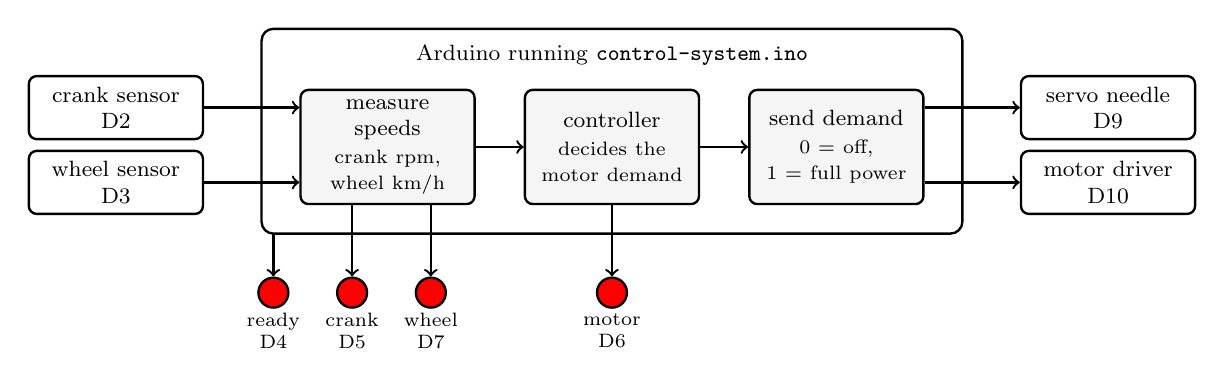
\begin{tikzpicture}[
    box/.style={draw, line width=.3mm, rounded corners=1mm, align=center,
        font=\footnotesize, inner sep=3pt},
    device/.style={box, text width=2cm, minimum height=.8cm},
    stage/.style={box, text width=2cm, minimum height=1.45cm,
        fill=black!4},
    arrow/.style={->, line width=.3mm},
    led/.style={circle, fill=red, draw=black, line width=.3mm,
        minimum size=.38cm, inner sep=0},
    ledname/.style={font=\scriptsize, align=center, anchor=north,
        inner sep=1pt},
]
    %% the Arduino, and the three stages of the sketch inside it
    \draw[line width=.3mm, rounded corners=1.5mm] (-4.45, -1.05)
        rectangle (4.45, 1.55);
    \node[font=\footnotesize] at (0, 1.22)
        {Arduino running \texttt{control-system.ino}};
    \node[stage] (measure) at (-2.85, .05)
        {measure\\speeds\\[2pt]{\scriptsize crank rpm,\\wheel km/h}};
    \node[stage] (control) at (0, .05)
        {controller\\[2pt]{\scriptsize decides the\\motor demand}};
    \node[stage] (send) at (2.85, .05)
        {send demand\\[2pt]{\scriptsize 0 = off,\\1 = full power}};
    \draw[arrow] (measure) -- (control);
    \draw[arrow] (control) -- (send);

    %% what goes in and what comes out
    \node[device] (crank) at (-6.3, .55) {crank sensor\\D2};
    \node[device] (wheel) at (-6.3, -.4) {wheel sensor\\D3};
    \node[device] (servo) at (6.3, .55) {servo needle\\D9};
    \node[device] (driver) at (6.3, -.4) {motor driver\\D10};
    \draw[arrow] (crank) -- (crank -| measure.west);
    \draw[arrow] (wheel) -- (wheel -| measure.west);
    \draw[arrow] (servo -| send.east) -- (servo);
    \draw[arrow] (driver -| send.east) -- (driver);

    %% the status LEDs, each fed by the part of the sketch that sets it
    \foreach \name/\pin/\x/\y in {ready/D4/-4.3/-1.05,
            crank/D5/-3.3/-.68, wheel/D7/-2.3/-.68,
            motor/D6/0/-.68}{
        \node[led] (led-\name) at (\x, -1.8) {};
        \draw[arrow] (\x, \y) -- (led-\name);
        \node[ledname] at (\x, -2.02) {\name\\\pin};
    }
\end{tikzpicture}
\end{document}
